\chapter{Electronic Structure}\label{ch:arpes}
In this brief chapter, we take a look at the Fermi surface as measured by Angle-Resolved Photoemission Spectroscopy (ARPES) on a sample of La$_2$CuO$_{4+\delta}$. Tha majority of the experimental work was performed with assistance from Johan Chang's group at the Laboratory for Quantum Matter Research (LQMR) in Z\"urich, Switzerland. I mention in particular Masafumi Horio, who helped me prepare the samples and did all of the data analysis. I was present at the measurements, but our success would not have been possible without the expertise of the LQMR group.

While the analysis presented here is \emph{very} preliminary, I include it because it is, to my knowledge, the first ARPES experiment performed on an oxygen doped La$_2$CuO$_{4+\delta}$ sample. Since these samples are known to phase separate (see XX) electronically, we expect a superposition of a magnetic `$\frac{1}{8}$' phase and an optimally superconducting phase. It is possible that we can see some of this behavior in an ARPES experiment.

\section{Sample}
The sample is a small piece ($\approx \SI{1}{\centi\meter\cubed}$) of La$_2$CuO$_{4+\delta}$, carefully cut with the $c$-axis vertical. Before cutting the sample, we characterized it with a Laue camera and magnetization measurements as shown in figure \ref{fig:arpes_vsm}. When performing ARPES experiments, you need an atomically flat surface. Since La$_2$CuO$_4$ is a very brittle material, the only way to do this is by gluing on a small pin, knocking it off and hoping that the sample breaks in an atomically sharp way. Luckily, the 2-dimensional nature of the cuprates also translate to their structural integrity, so they are likely to cleave naturally at the CuO$_2$ interface. Before going to the ARPES experiment, the procedure was tested in the lab as shown in figure \ref{fig:arpes_cleave}.

\begin{figure}
    \centering
    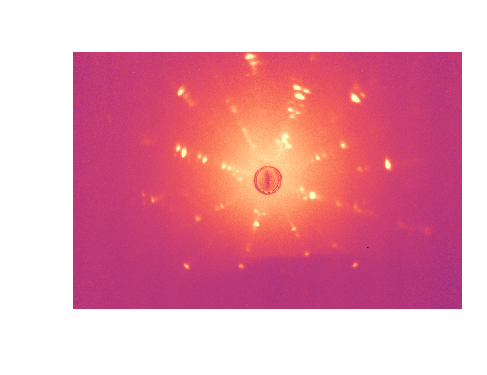
\includegraphics[width=0.49\textwidth]{fig/arpes/laue2.png}
    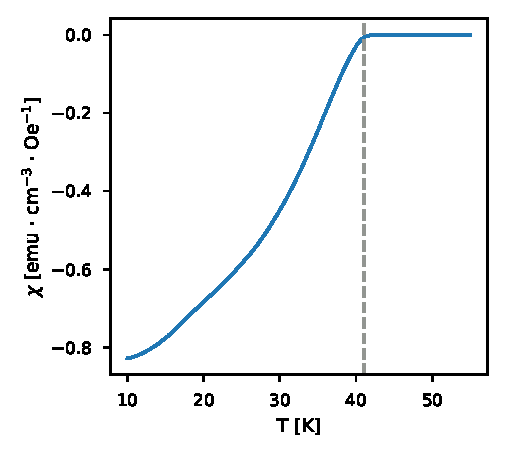
\includegraphics[width=0.49\textwidth]{fig/arpes/vsm_lcoo.pdf}
    \caption{\textbf{Left:} Laue diffraction pattern of the La$_2$CuO$_{4+\delta}$ sample, aligned with the $c$ axis vertical. \textbf{Right:} Vibrating Sample Magnetometry (VSM) performed on a Quantum Design MPMS. Normalization performed through $\chi=4\pi \frac{\mu(1-N)}{VH_\text{app}}$, where $\mu$ is the measured signal, $V$ is the volume, $H_\text{app}$ is the applied field and $N$ is the demagnetization factor. Vertical line marks the onset superconducting transition temperature $T_\text{c} = \SI{41}{\kelvin}$}
    \label{fig:arpes_vsm}
\end{figure}

\begin{figure}
    \centering
    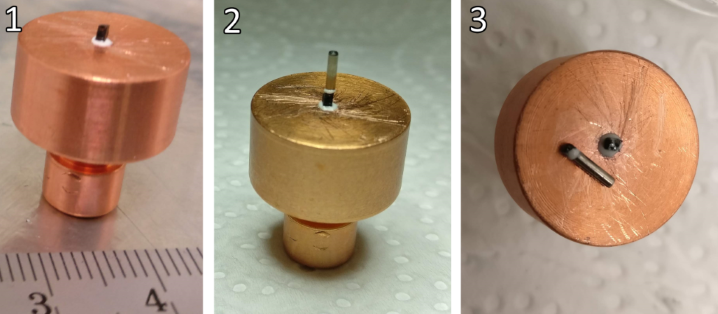
\includegraphics[width=0.8\textwidth]{fig/arpes/cleave.png}
    \caption{Cleaving procedure. \textbf{1:} The sample is mounted using Torr Seal Low Pressure Epoxy. \textbf{2:} A stainless steel pin ($L=6\,\text{mm}$, $d=1\,\text{mm}$) is glued to the top of the sample and subsequently \textbf{3:} knocked off with a regular screwdriver.}
    \label{fig:arpes_cleave}
\end{figure}


\section{Experiment}
ARPES experiments were carried out on the La$_2$CuO$_{4+\delta}$ sample at the Surface/Interface Spectroscopy (SIS) beamline at the Swiss Light Source. The sample was cleaved in situ at $\approx 20\,\text{K}$ under ultra high vacuum ($\leq 5 \times 10^{-11}\,\text{Torr}$) by employing the top-post technique as shown in figure \ref{fig:arpes_cleave}. Ultraviolet ARPES spectra were recorded using a SCIENTA R4000 electron analyser with horizontal slit setting. All the data were recorded at the cleaving temperature. Figure \ref{fig:arpes_fs} shows the Fermi surface map at $T=22\,\text{K}$ recorded using circularly polarized $160\,\text{eV}$ phonons.  Detailed cuts along the nodal directions with circularly polarized light is shown in Figure \ref{fig:arpes_cut1}. A comparison of different photon polarizations is shown in Figure \ref{fig:arpes_cut2}.

\begin{figure}
    \centering
    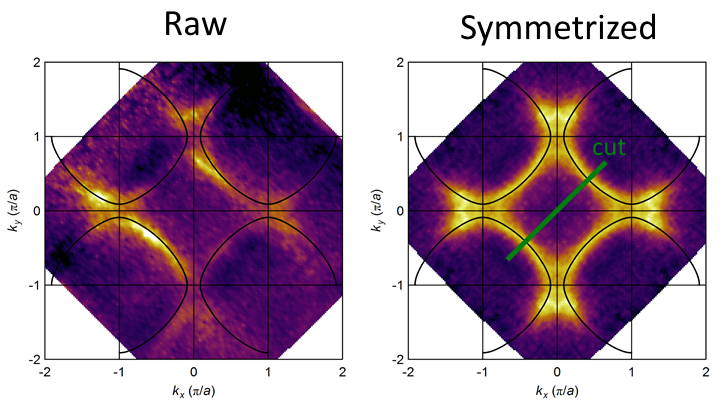
\includegraphics[width=0.8\textwidth]{fig/arpes/fermi_surface.png}
    \caption{Fermi surface of at $22\,\text{K}$ represented as raw and symmetrized data. $k_x$ and $k_y$ are in tetragonal (I4/mmm) units. The cut indicates the nodal direction as used in subsequent measurements of the band structure.}
    \label{fig:arpes_fs}
\end{figure}

\section{Discussion}
The area of the Fermi surface as shown in Figure \ref{fig:arpes_fs} corresponds to a carrier (hole) doping $n_\text{h} = 0.16$ and a hopping parameter $\frac{t^\prime}{t} \approx -0.14$, according to analysis performed by Masafumi Horio from the LMQR group.
It turns out that the measured spectra as e.g. the cut shown in Figure \ref{fig:arpes_cut1} are very similar to what was observed by the LMQR group in overdoped La$_{1.77}$Sr$_{0.23}$CuO$_4$ \cite{Horio2018}. There is thus no indication of `$\frac{1}{8}$-physics' which is generally characterized by the formation of Fermi arcs. We cannot however rule out that such arcs are not observed due to an unfavourable superposition of photoemission from the 1/8 phase and optimally doped phase in our sample.  

\begin{figure}
    \centering
    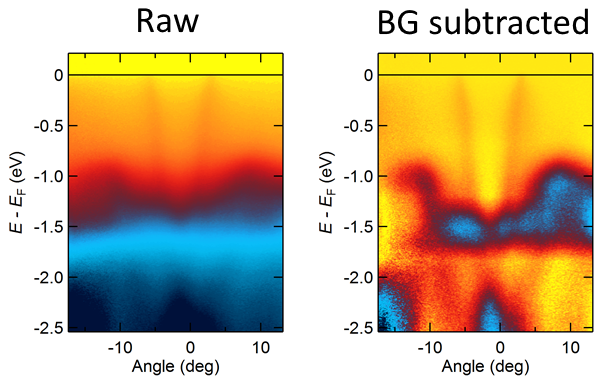
\includegraphics[width=0.8\textwidth]{fig/arpes/hs_cut1.png}
    \caption{Cut along the nodal direction (see Figure \ref{fig:arpes_fs}) with 160 eV circularly polarized photons. The subtracted background is defined by the minimum Momentum Distribution Curve (MDC) intensity at each binding energy.}
    \label{fig:arpes_cut1}
\end{figure}

Figure \ref{fig:arpes_cut2} clearly shows that we can separate the $d_{x^2-y^2}$ band from the $d_z$ band using different polarizations of light. When comparing to overdoped La$_{1.77}$Sr$_{0.23}$CuO$_4$, the band structure is very similar except that the $d_z$ band is moved down by about $\SI{0.1}{\eV}$. This could be due to an elongation of the $c$-axis, but while oxygen-doped samples are elongated when compared to the parent compound, La$_2$CuO$_{4+\delta}$ has a similar (or even smaller) $c$-axis when compared to La$_{1.77}$Sr$_{0.23}$CuO$_4$.

\begin{figure}
    \centering
    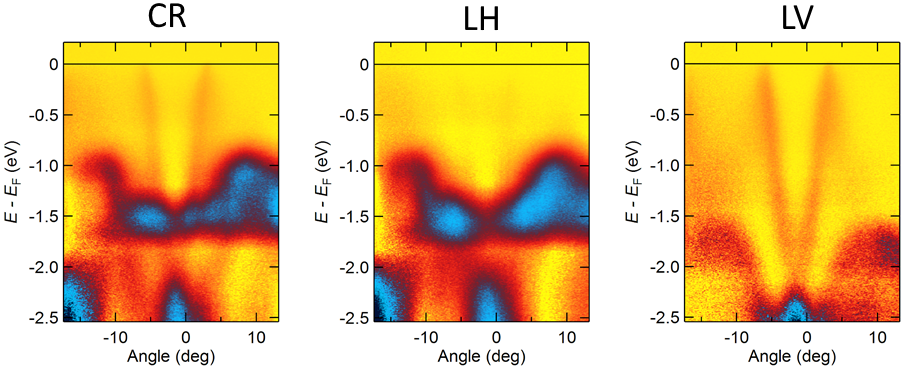
\includegraphics[width=\textwidth]{fig/arpes/hs_cut2.png}
    \caption{Cut along the nodal direction (see Figure \ref{fig:arpes_fs}) with 160 eV circular (CR), linear horizontal (LH) and linear vertical (LV) polarized photons.}
    \label{fig:arpes_cut2}
\end{figure}